\documentclass[conference]{IEEEtran}
\IEEEoverridecommandlockouts

\usepackage{cite}
\usepackage{amsmath,amssymb}
\usepackage{graphicx}
\usepackage{booktabs}
\usepackage{array}
\usepackage{tabularx}
\usepackage{url}
\usepackage{balance}

\graphicspath{{final_artifacts/assets/}{../TSFFM-Depression-Detection/results/}}

\newcommand{\gap}{\textbf{[INCOMPLETE DATA GAP]}}
\newcolumntype{Y}{>{\raggedright\arraybackslash}X}

\begin{document}

\title{Visual Landmark-Based Two-Stream Temporal Fusion for AI-Assisted Depression Screening from Interview Video}

\author{
\IEEEauthorblockN{Jitendra Choudhary\IEEEauthorrefmark{1}, Kabir Singh Khair\IEEEauthorrefmark{1}}
\IEEEauthorblockA{\IEEEauthorrefmark{1}Department of Electronics and Communication Engineering\\
PDPM Indian Institute of Information Technology, Design and Manufacturing, Jabalpur, India\\
Supervisor: Dr. Amit Vishwakarma}
}

\maketitle

\begin{abstract}
Depression screening commonly depends on clinical interviews, questionnaires, and professional interpretation. These methods remain necessary, but access constraints and under-reporting motivate assistive tools that can analyze behavioral evidence in a repeatable manner. This paper presents a final-year project prototype for AI-assisted depression screening from interview video using a landmark-based Two-Stream Feature Fusion Model (TSFFM). The implemented system extracts a 68-point facial landmark subset using MediaPipe FaceMesh and shoulder-level pose landmarks using MediaPipe Pose. The features are normalized, sampled to a fixed 360-frame sequence, projected through separate face and body streams, fused into a 160-dimensional temporal representation, smoothed by a one-dimensional temporal convolution, and classified by a bidirectional LSTM with temporal attention. The model is integrated into a FastAPI backend and React/Vite frontend that supports video upload, probability display, detection-quality reporting, and PDF report generation. On the available validation evaluation, the selected checkpoint achieved 57.67\% accuracy, 0.4688 precision, 0.4255 recall, 0.4461 F1-score, and 0.6597 AUC-ROC over 352 segments. A recall-oriented candidate achieved 0.8227 recall and 0.5873 F1-score but lower accuracy and AUC. The results indicate that the prototype learns measurable signal but is not clinically ready. The main contributions are an end-to-end visual screening workflow, an implementation-grounded two-stream temporal architecture, and a transparent analysis of limitations, including missing external validation, limited pose representation, and absent clinical calibration.
\end{abstract}

\begin{IEEEkeywords}
Depression screening, behavioral computing, facial landmarks, pose landmarks, temporal attention, LSTM, multimodal fusion, DAIC-WOZ, FastAPI.
\end{IEEEkeywords}

\section{Introduction}
Depression is a major public-health concern. The World Health Organization reports that approximately 332 million people worldwide have depression, with prevalence varying across age and demographic groups \cite{who_depression}. Screening and diagnosis remain clinical tasks, typically conducted through interview, questionnaire, and professional judgment. However, access limitations, stigma, and self-report bias can delay care. Automated behavioral analysis can therefore be useful as an assistive screening component, provided that its limitations are explicitly stated and clinical decision-making remains with qualified professionals.

Video interviews contain non-verbal signals that may be relevant to depression assessment, including facial expressiveness, gaze behavior, posture, and psychomotor activity. Prior depression-recognition research has frequently used the DAIC-WOZ and AVEC challenge settings, where audio, video, and transcript modalities are collected during human--computer or semi-clinical interviews \cite{gratch_daic, ringeval_avec2017, zhang_multimodal}. These datasets support reproducible experimentation, but they are small relative to modern deep-learning requirements, and generalization across cohorts remains difficult.

The project reported in this paper began as a mid-semester TSFFM concept centered on two visual streams: a facial stream and a body-posture stream. The final implementation changes the early frame-level CNN concept into a compact landmark-based temporal architecture. Specifically, the deployed pipeline extracts face and pose coordinate features, normalizes them, uses separate multilayer streams for face and body, fuses the streams, and uses bidirectional temporal modeling with attention. The model is connected to a complete web application with backend inference and automatic PDF report generation.

This paper is evidence-driven and does not claim clinical validity. Quantitative results are limited to the available validation output saved in the project repository. No external clinical trial, participant-level fairness audit, or deployment hardware benchmark is available. These gaps are explicitly identified rather than inferred.

\section{Related Work}
\subsection{Depression Interview Corpora and Benchmarks}
The Distress Analysis Interview Corpus (DAIC) contains clinical interviews designed to support the diagnosis of psychological distress conditions such as depression, anxiety, and post-traumatic stress disorder \cite{gratch_daic}. The DAIC-WOZ depression database documentation describes Wizard-of-Oz interviews conducted by a virtual interviewer and includes audio, video, questionnaire responses, and transcribed/annotated features \cite{daic_doc}. AVEC 2017 provided benchmark conditions for affect and depression analysis using common data and evaluation procedures \cite{ringeval_avec2017}. These benchmark settings motivate this project because they frame depression detection as a multimodal behavioral-computing problem rather than as a conventional image-classification task.

\subsection{Visual Landmark Extraction}
MediaPipe FaceMesh is related to real-time facial surface geometry estimation from monocular video, where dense face meshes are inferred efficiently on mobile hardware \cite{kartynnik_facemesh}. MediaPipe Pose and BlazePose-style systems provide body landmarks suitable for real-time human pose estimation \cite{grishchenko_blazepose}. The current prototype uses these tools as deterministic feature extractors rather than training an image-to-depression network directly.

\subsection{Temporal Modeling and Class Imbalance}
Depression-related behavior is temporal. LSTM networks were introduced to address long-term dependency learning in recurrent neural networks \cite{hochreiter_lstm}. This project uses a bidirectional LSTM to model the fixed-length landmark sequence. Class imbalance is addressed using class weights, weighted sampling, and focal loss. Focal loss was originally proposed for dense object detection to down-weight well-classified examples and emphasize harder examples \cite{lin_focal}. In this project, focal loss is used as a training choice for imbalanced binary screening, not as evidence of clinical robustness.

\begin{table*}[t]
\caption{Literature Review and Relevance to the Present TSFFM Prototype}
\label{tab:litreview}
\centering
\begin{tabularx}{\textwidth}{p{0.20\textwidth}Y Y Y}
\toprule
\textbf{Paper or Source} & \textbf{Contribution} & \textbf{Limitation} & \textbf{Relevance to TSFFM} \\
\midrule
Gratch et al. \cite{gratch_daic} & Introduced DAIC, a corpus of clinical interviews containing verbal and non-verbal indicators of psychological distress. & Dataset access and partitioning constraints limit direct replication without the full corpus. & Defines the interview-based behavioral setting used by many depression-detection systems. \\
Ringeval et al. \cite{ringeval_avec2017} & Established AVEC 2017 benchmark conditions for real-life depression and affect recognition. & Challenge baselines do not remove the need for independent validation on new cohorts. & Provides the evaluation context for multimodal depression detection. \\
Zhang et al. \cite{zhang_multimodal} & Demonstrated multimodal depression detection and assessment using text, audio, and video on DAIC-WOZ. & Uses modalities beyond the current project; direct comparison is not valid without matching splits and inputs. & Shows why extending TSFFM with audio and text is a strong future direction. \\
Kartynnik et al. \cite{kartynnik_facemesh} & Presented real-time facial surface geometry estimation from monocular video. & Designed for face geometry, not clinical inference. & Supports the use of facial landmarks as compact visual descriptors. \\
Grishchenko et al. \cite{grishchenko_blazepose} & Presented real-time 3D body landmarks and pose estimation. & Pose accuracy does not imply depression-detection validity. & Supports body-landmark extraction for posture and motion cues. \\
Hochreiter and Schmidhuber \cite{hochreiter_lstm} & Introduced LSTM for long-range temporal dependency modeling. & LSTM alone does not solve small-data generalization. & Justifies temporal modeling beyond frame-level classification. \\
Lin et al. \cite{lin_focal} & Introduced focal loss to address severe class imbalance during training. & Proposed for object detection; transfer to depression screening requires validation. & Motivates the repository's focal-loss training option for imbalanced classes. \\
\bottomrule
\end{tabularx}
\end{table*}

\section{Architecture Analysis}
This section follows an implementation-evidence structure: components, data flow, control flow, communication flow, safety mechanisms, and code-backed evidence.

\subsection{Components}
The implemented system consists of six main components:
\begin{enumerate}
\item \textbf{Frontend dashboard}: a React/Vite interface for video upload, patient/session metadata entry, loading-state display, result visualization, and PDF report download.
\item \textbf{Prediction API}: a FastAPI route at \texttt{/api/predict} that validates uploads, invokes feature extraction, runs inference, and returns structured JSON.
\item \textbf{Feature extractor}: an OpenCV and MediaPipe service that samples video frames, extracts face and pose landmarks, normalizes them, and returns fixed-length feature arrays.
\item \textbf{TSFFM temporal model}: a PyTorch model with face stream, body stream, temporal convolution, bidirectional LSTM, temporal attention, and binary classifier.
\item \textbf{Training and evaluation scripts}: PyTorch scripts for training, checkpointing, metric computation, and plot generation.
\item \textbf{Report generator}: a ReportLab service that writes a PDF report containing metadata, prediction, confidence values, probabilities, processing details, and disclaimer text.
\end{enumerate}

\subsection{Data Flow}
The deployed data flow begins with an uploaded video file. The backend stores it temporarily, samples frames at 5 FPS, extracts facial and shoulder pose landmarks, pads or truncates the sequence to 360 frames, normalizes coordinates per frame, flattens the face sequence to shape \(360 \times 272\), flattens the pose sequence to shape \(360 \times 8\), and converts both arrays into tensors with batch dimension. The model produces logits for two classes: not depressed and depressed. A softmax layer produces probabilities that are returned to the frontend and inserted into the generated report.

\begin{figure}[t]
\centering
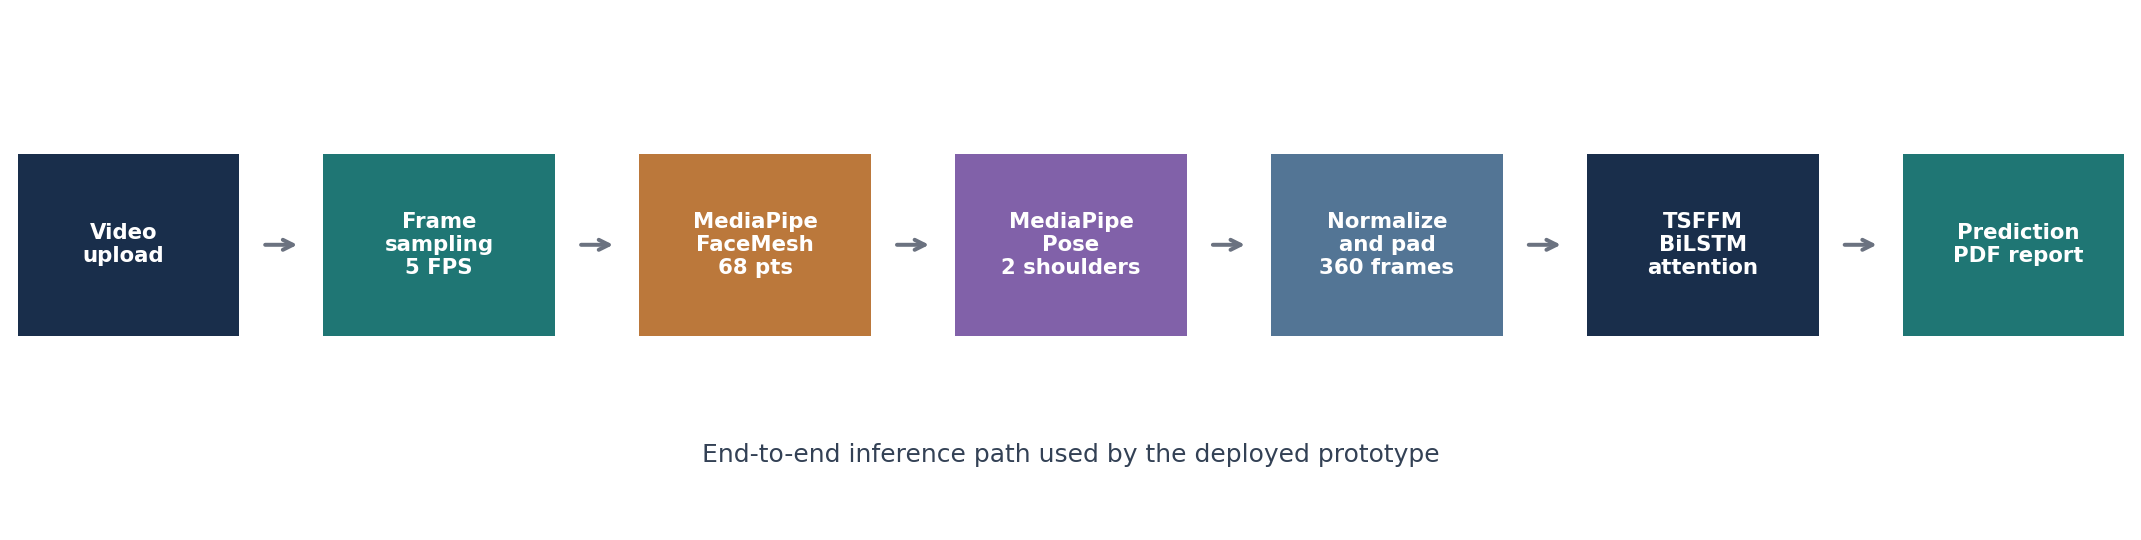
\includegraphics[width=\linewidth]{system_pipeline.png}
\caption{End-to-end inference pipeline implemented in the project. The diagram is generated from repository evidence and uses the actual deployed sequence length and feature dimensions.}
\label{fig:pipeline}
\end{figure}

\subsection{Control Flow}
The control flow is request-driven. A frontend upload event triggers a POST request to \texttt{/api/predict}. The backend validates the extension against allowed video formats, saves the upload, extracts features, loads or reuses the cached PyTorch model singleton, computes probabilities, generates a report, returns a JSON response, and attempts temporary-file cleanup. Exceptions during video processing are converted into HTTP 500 responses with an error message.

\subsection{Communication Flow}
Frontend--backend communication occurs through HTTP multipart form upload. The request includes a video file, patient identifier, and session date. The response includes prediction, confidence, depressed probability, not-depressed probability, face detection rate, body detection rate, processing time, frames processed, sampled frames, sequence length, and report URL. The report URL points to a statically mounted backend reports directory.

\subsection{Safety Mechanisms}
The implemented safety mechanisms are primarily software and communication safeguards, not clinical safeguards. File extensions are checked before processing. Uploaded files are deleted in a \texttt{finally} block after inference. The generated report contains a medical disclaimer. The frontend and report text state that the system is a screening prototype rather than a diagnosis tool.

\gap{} Quantitative evidence is unavailable for adversarial upload handling, privacy compliance, encryption, retention-policy enforcement, subgroup fairness, model calibration, or clinical review.

\subsection{Implementation Evidence}
\begin{table}[t]
\caption{Repository Evidence for the Implemented Architecture}
\label{tab:impl_evidence}
\centering
\begin{tabularx}{\linewidth}{p{0.28\linewidth}Y}
\toprule
\textbf{File} & \textbf{Evidence} \\
\midrule
\texttt{backend/api/predict.py} & Implements upload validation, temporary save, feature extraction, inference, PDF generation, JSON response, and cleanup. \\
\texttt{backend/services/extractor.py} & Implements OpenCV video reading, MediaPipe FaceMesh and Pose extraction, 68-face-landmark subset, two-shoulder pose features, normalization, padding/truncation, and metadata. \\
\texttt{backend/services/inference.py} & Loads \texttt{TSFFM\_LSTM}, restores weights when available, applies softmax, and returns prediction and confidence. \\
\texttt{ml/models.py} & Defines face stream, body stream, temporal convolution, bidirectional LSTM, temporal attention, and classifier. \\
\texttt{ml/train.py} & Defines focal loss, class weights, balanced sampler, Adam optimizer, LR scheduling, gradient clipping, early stopping, and history logging. \\
\texttt{ml/evaluate.py} & Computes accuracy, precision, recall, F1-score, AUC-ROC, classification report, confusion matrix, ROC curve, and history plots. \\
\texttt{frontend/src/App.jsx} & Coordinates dashboard tabs, upload workflow, loading stages, result state, error state, and model information view. \\
\texttt{frontend/src/components/UploadBox.jsx} & Implements upload UI, file format validation, patient/session metadata input, and submission. \\
\texttt{frontend/src/components/ResultCard.jsx} & Displays prediction, confidence, class probabilities, report link, and clinical note/disclaimer language. \\
\bottomrule
\end{tabularx}
\end{table}

\section{Methodology}
\subsection{Feature Extraction}
For each sampled frame, FaceMesh produces dense facial landmarks. The implementation selects 68 indices to form a standard facial subset. Each facial point stores \(x\), \(y\), \(z\), and confidence, yielding \(68 \times 4 = 272\) values per frame. Pose extraction uses the left and right shoulders from MediaPipe Pose; each point stores \(x\), \(y\), \(z\), and visibility, yielding \(2 \times 4 = 8\) values per frame.

Each sequence is centered by subtracting the per-frame mean over spatial coordinates. It is scaled by the maximum per-frame distance from the center, with zero-distance protection. Videos shorter than the target length are padded by repeating the last available frame; longer videos are truncated to 360 sampled frames. If no readable frames exist, zero arrays are returned. If a face or pose is missing after prior detections, the last detected feature frame is reused.

\subsection{Model}
Let \(F \in \mathbb{R}^{T \times 272}\) denote the facial sequence and \(P \in \mathbb{R}^{T \times 8}\) denote the pose sequence, where \(T=360\). The face stream maps each \(272\)-dimensional vector to a 128-dimensional latent representation through linear layers, batch normalization, ReLU activation, and dropout. The body stream maps each \(8\)-dimensional pose vector to a 32-dimensional representation using a similar multilayer projection. The features are concatenated into \(X \in \mathbb{R}^{T \times 160}\).

A one-dimensional convolution with kernel size 3 is applied over the temporal dimension. A bidirectional LSTM then maps the fused sequence into hidden states. Temporal attention computes scalar weights over LSTM outputs and forms a context vector by weighted summation. A final fully connected classifier produces two logits.

\begin{figure}[t]
\centering
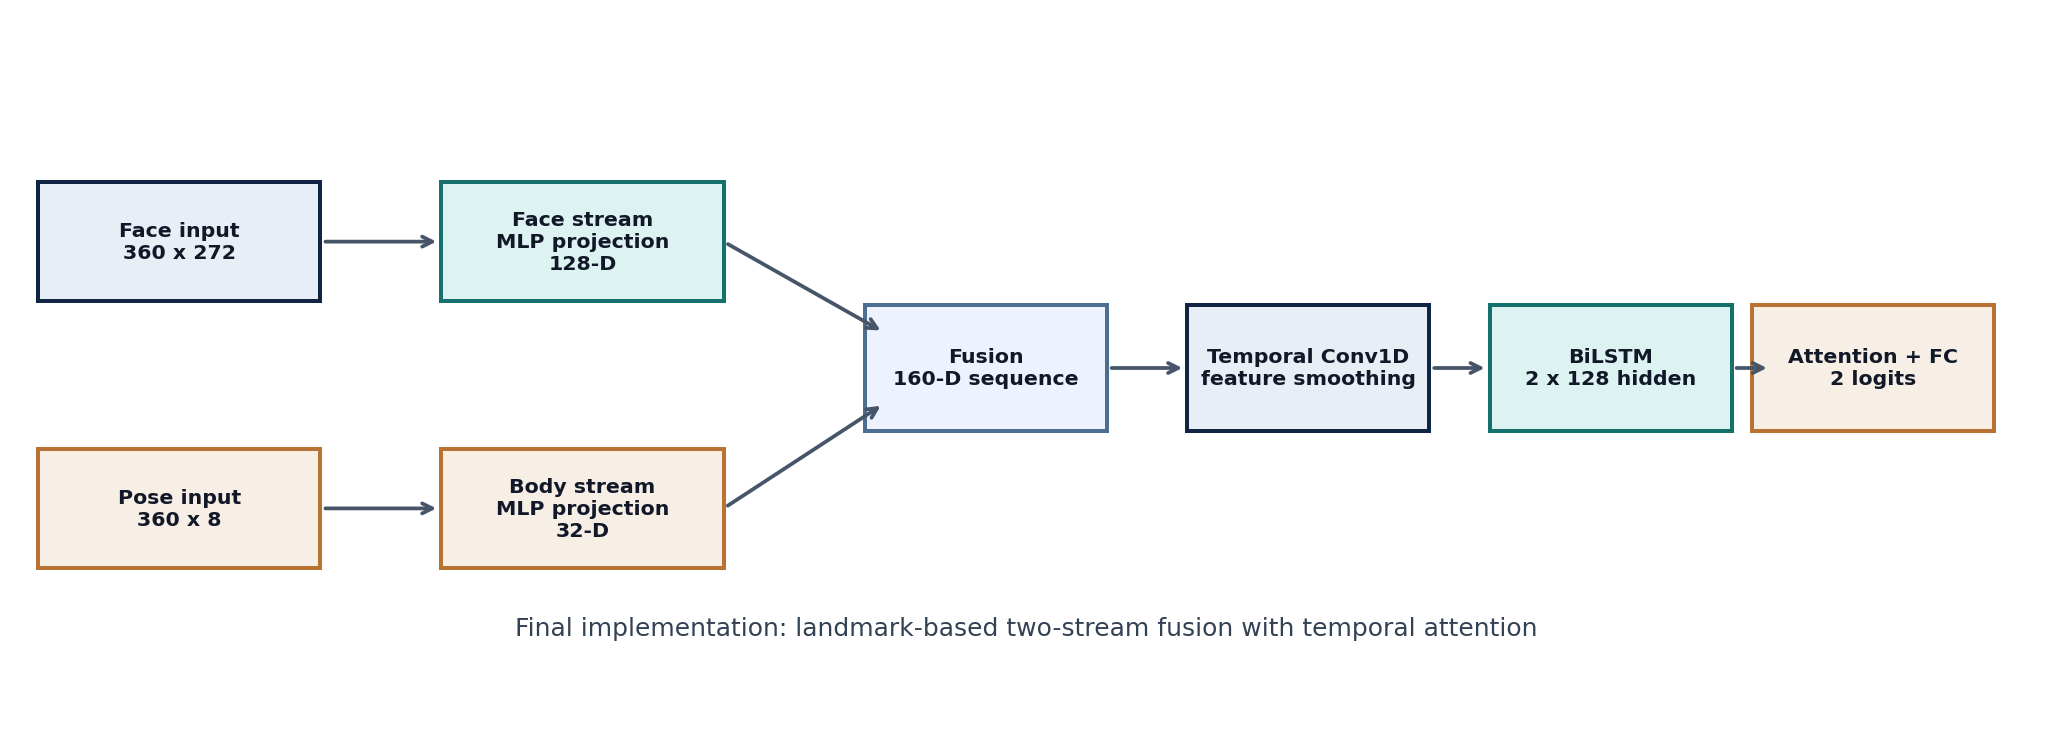
\includegraphics[width=\linewidth]{model_architecture.png}
\caption{Implemented TSFFM temporal architecture. The final code uses landmark feature projection rather than the mid-semester image-CNN design.}
\label{fig:model}
\end{figure}

\subsection{Training}
The training script uses Adam optimization with weight decay. Class imbalance is handled with class weights and a weighted random sampler. The default loss option in the final training script is focal loss with \(\gamma=2\). The script logs loss, accuracy, precision, recall, F1-score, AUC, and learning rate. Checkpointing is based on a selected validation metric, and early stopping is triggered when improvement stalls.

\gap{} The repository evidence does not provide a complete experiment ledger describing exact hardware, wall-clock training time, random-seed repetitions, or participant-level split verification. The code sets a random seed, but a single saved result cannot establish variance across repeated runs.

\section{Experimental Analysis}
\subsection{Evaluation Protocol}
The evaluation script loads the validation split, restores the trained checkpoint, performs inference, and computes accuracy, precision, recall, F1-score, and AUC-ROC. It also saves a text classification report, confusion matrix figure, ROC curve, and training-history plots.

\begin{table}[t]
\caption{Experimental Evidence Available in the Repository}
\label{tab:experiments}
\centering
\begin{tabularx}{\linewidth}{p{0.26\linewidth}Y Y Y}
\toprule
\textbf{Experiment} & \textbf{Evidence} & \textbf{Result} & \textbf{Limitation} \\
\midrule
Selected checkpoint validation & \texttt{results/classification\_report.txt} & 57.67\% accuracy, 0.4461 F1, 0.6597 AUC & Validation only; no external test-set evidence. \\
Recall-oriented candidate & \texttt{results/retrained\_candidate/classification\_report.txt} & 0.8227 recall, 0.5873 F1, 0.5454 AUC & Higher sensitivity but weaker ranking quality and accuracy. \\
Training dynamics & \texttt{backend/weights/training\_history.json}, \texttt{accuracy\_history.png}, \texttt{loss\_history.png} & Training improves more strongly than validation & Indicates overfitting pressure; no repeated-run variance. \\
Confusion behavior & \texttt{confusion\_matrix.png} and class report & More reliable not-depressed recognition than depressed recognition in selected checkpoint & Exact threshold calibration not reported. \\
End-to-end application path & Backend reports and frontend/backend source & Upload, inference, result display, and PDF generation implemented & No quantified latency or usability study. \\
\bottomrule
\end{tabularx}
\end{table}

\subsection{Quantitative Results}
\begin{table}[t]
\caption{Validation Results from Repository Artifacts}
\label{tab:metrics}
\centering
\begin{tabular}{lccccc}
\toprule
\textbf{Model} & \textbf{Acc.} & \textbf{Prec.} & \textbf{Rec.} & \textbf{F1} & \textbf{AUC} \\
\midrule
Selected checkpoint & 57.67 & 0.4688 & 0.4255 & 0.4461 & 0.6597 \\
Recall-oriented candidate & 53.69 & 0.4567 & 0.8227 & 0.5873 & 0.5454 \\
\bottomrule
\end{tabular}
\end{table}

Table~\ref{tab:metrics} shows that the selected checkpoint has the stronger AUC-ROC and accuracy, while the recall-oriented candidate detects a larger fraction of depressed samples at the cost of ranking quality and overall accuracy. In a screening setting, recall is important because false negatives are harmful. However, a high-recall operating point must be calibrated with clinical input to manage false-positive burden.

\begin{figure}[t]
\centering
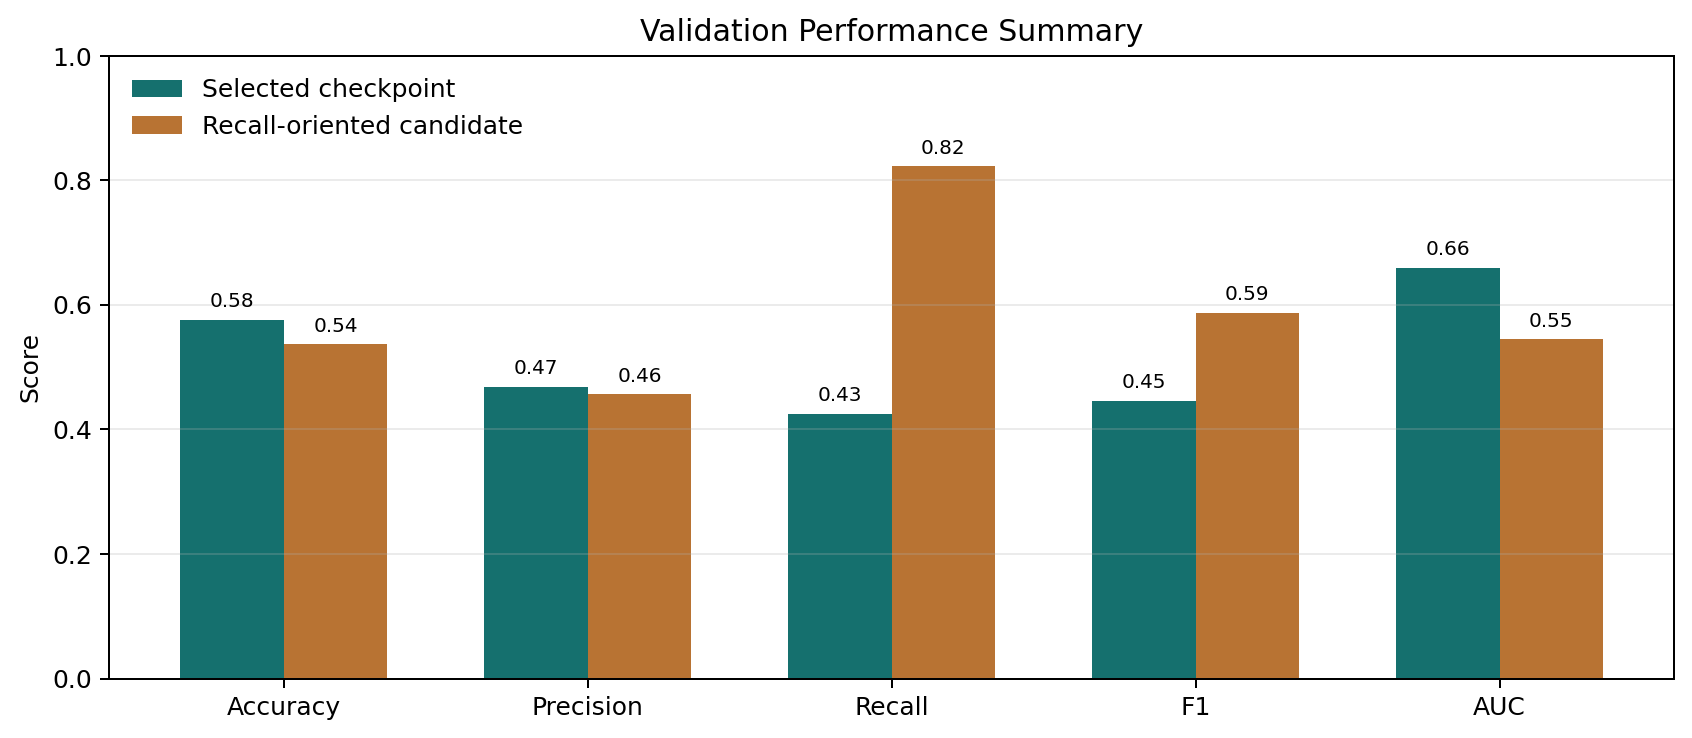
\includegraphics[width=\linewidth]{metrics_summary.png}
\caption{Metric comparison between the selected checkpoint and recall-oriented candidate.}
\label{fig:metrics}
\end{figure}

\subsection{Class-Level Interpretation}
The selected checkpoint classification report includes 211 not-depressed validation segments and 141 depressed validation segments. The not-depressed class achieved 0.64 precision, 0.68 recall, and 0.66 F1-score. The depressed class achieved 0.47 precision, 0.43 recall, and 0.45 F1-score. The lower depressed-class recall is a major concern for an assistive screening system.

\begin{figure}[t]
\centering

\includegraphics[width=0.90\linewidth]{confusion_matrix.png}
\caption{Confusion matrix saved by the evaluation script for the selected checkpoint.}
\label{fig:cm}
\end{figure}

\begin{figure}[t]
\centering

\includegraphics[width=0.90\linewidth]{roc_curve.png}
\caption{ROC curve saved by the evaluation script. The reported AUC-ROC is 0.6597.}
\label{fig:roc}
\end{figure}

\subsection{Training Dynamics}
The logged training history shows that training accuracy rises to the mid-80\% range, while validation accuracy remains near the low-to-mid 50\% range across later epochs. This gap suggests overfitting pressure. It is consistent with the expected difficulty of small behavioral datasets and supports the need for stronger regularization, richer data, and external validation.

\begin{figure}[t]
\centering
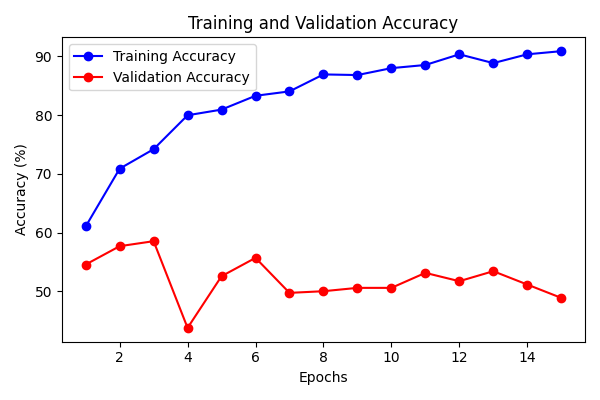
\includegraphics[width=0.90\linewidth]{accuracy_history.png}
\caption{Training and validation accuracy history generated by the evaluation script.}
\label{fig:acc}
\end{figure}

\begin{figure}[t]
\centering

\includegraphics[width=0.90\linewidth]{loss_history.png}
\caption{Training and validation loss history generated by the evaluation script.}
\label{fig:loss}
\end{figure}

\section{Discussion}
The final prototype demonstrates a functioning end-to-end visual screening system. Its main engineering improvement over the mid-semester version is the transition from a conceptual two-stream slide model to a deployed temporal pipeline with feature extraction, model inference, frontend interaction, probability display, and report generation. The main research improvement is the addition of bidirectional temporal modeling and attention.

The quantitative results do not support a clinical deployment claim. The selected checkpoint's AUC-ROC of 0.6597 suggests that the probability scores contain some discriminative information, but the depressed-class recall of 0.4255 is not acceptable for a high-sensitivity screening use case without further calibration and validation. The recall-oriented candidate demonstrates that sensitivity can be increased, but its lower AUC-ROC suggests that the classifier's ranking quality is unstable.

The deployed body stream is also narrower than the original mid-semester concept. The mid-semester deck described 33 body landmarks and a 132-dimensional pose vector; the final implementation uses only two shoulder landmarks and an 8-dimensional pose vector. This is a verified implementation difference and should be described transparently. The limited pose representation may reduce the model's ability to detect whole-body psychomotor behavior.

\section{Ethics, Privacy, and Clinical Safety}
This system processes interview video, which is sensitive behavioral and biometric data. Any deployment outside a controlled academic demonstration would require informed consent, secure storage, retention limits, access control, and ethics approval. The generated reports must not be treated as medical diagnoses.

The prototype should be restricted to research and educational screening demonstrations unless clinically validated. The appropriate human-in-the-loop interpretation is: a model output may suggest whether further professional screening is warranted, but it must not determine diagnosis, treatment, employment, insurance, or disciplinary decisions.

\gap{} No evidence is available for clinical review, institutional ethics approval, subgroup fairness testing, cross-cultural validation, or privacy-law compliance. These missing elements are blocking concerns for any real deployment.

\section{Limitations}
\begin{enumerate}
\item \textbf{Validation scope}: results are available for the repository's validation evaluation, not for an external held-out clinical cohort.
\item \textbf{Data provenance}: the code references DAIC-WOZ/E-DAIC style pre-extracted features, but the exact local dataset copy, participant list, and participant-level split audit are not documented in the repository artifacts used here.
\item \textbf{Pose representation}: the deployed extractor uses only left and right shoulder landmarks, which under-represents body motion.
\item \textbf{No ablation study}: there is no code-backed ablation separating face-only, body-only, fusion-only, BiLSTM-only, and attention variants.
\item \textbf{No repeated-run statistics}: only saved metric outputs are available; confidence intervals and seed variance are not reported.
\item \textbf{No calibration analysis}: no threshold sweep, reliability diagram, or clinical operating point selection is available.
\item \textbf{No latency benchmark}: the web system is implemented, but quantitative runtime evidence is unavailable.
\item \textbf{No clinical validation}: no psychiatrist-reviewed trial or PHQ-9/DSM-5 clinical assessment study is documented.
\item \textbf{Model-version consistency}: the current \texttt{ml/evaluate.py} source instantiates \texttt{TSFFM\_LSTM} with one LSTM layer, whereas \texttt{ml/train.py} and \texttt{backend/services/inference.py} instantiate the model with two LSTM layers. The saved metric files are reported as repository artifacts, but exact reproduction requires aligning these scripts.
\end{enumerate}

\section{Future Work}
The most important next step is to improve validation quality before model complexity. A publishable extension should include participant-level split documentation, external test evaluation, repeated runs with confidence intervals, and ablations for face stream, pose stream, fusion, temporal convolution, LSTM, and attention.

The model should also be extended to richer multimodal evidence. Audio prosody, pause duration, speech rate, and transcript semantics are strongly relevant to depression interviews and are used in prior DAIC-WOZ studies \cite{zhang_multimodal}. A tri-stream architecture combining visual landmarks, acoustic descriptors, and transcript embeddings would better match the multimodal nature of clinical interviews. Probability calibration and threshold selection should be performed with domain experts.

\section{Conclusion}
This paper presented an implementation-grounded TSFFM prototype for AI-assisted depression screening from interview video. The system extracts visual landmarks, fuses facial and pose streams, models temporal behavior with a bidirectional LSTM and attention, and exposes the model through a web application with report generation. The final implementation is stronger and more complete than the mid-semester concept because it connects model development to a usable workflow.

The current evidence supports the claim that the prototype functions end to end and learns measurable validation signal. It does not support claims of clinical readiness, generalizable diagnostic performance, or deployment safety. The selected checkpoint achieved 57.67\% validation accuracy and 0.6597 AUC-ROC, while the recall-oriented candidate achieved higher recall but lower AUC. Therefore, the system is best characterized as a research prototype requiring stronger data, ablation, calibration, and clinical validation before practical use.

\section*{Reproducibility Statement}
The manuscript is based on repository files available in the local project folder, the extracted mid-semester presentation text, saved evaluation reports, saved training history, and generated plots. Quantitative evidence unavailable in these files is not inferred. \gap{} The exact external dataset copy, hardware runtime, clinical approval, and repeated-run variance are not documented in the evidence available for this manuscript.

\section*{Medical Disclaimer}
The system described here is an AI-assisted screening prototype. It is not a diagnostic device and must not be used for medical decisions without professional clinical validation and qualified mental-health oversight.

\balance

\begin{thebibliography}{00}
\bibitem{who_depression}
World Health Organization, ``Depressive disorder (depression),'' Aug. 29, 2025. [Online]. Available: \url{https://www.who.int/news-room/fact-sheets/detail/depression}. Accessed: Jun. 7, 2026.

\bibitem{gratch_daic}
J. Gratch, R. Artstein, G. Lucas, G. Stratou, S. Scherer, A. Nazarian, R. Wood, J. Boberg, D. DeVault, S. Marsella, D. Traum, A. Rizzo, and L.-P. Morency, ``The Distress Analysis Interview Corpus of human and computer interviews,'' in \emph{Proc. 9th Int. Conf. Language Resources and Evaluation (LREC)}, 2014.

\bibitem{daic_doc}
USC Institute for Creative Technologies, ``DAIC-WOZ Depression Database: Documentation for AVEC 2017,'' 2017. [Online]. Available: \url{https://dcapswoz.ict.usc.edu/wwwdaicwoz/DAICWOZDepression_Documentation_AVEC2017.pdf}. Accessed: Jun. 7, 2026.

\bibitem{ringeval_avec2017}
F. Ringeval, B. Schuller, M. Valstar, J. Gratch, R. Cowie, S. Scherer, S. Mozgai, N. Cummins, M. Schmitt, and M. Pantic, ``AVEC 2017: Real-life depression, and affect recognition workshop and challenge,'' in \emph{Proc. 7th Annu. Workshop Audio/Visual Emotion Challenge}, 2017, pp. 3--9, doi: 10.1145/3133944.3133953.

\bibitem{zhang_multimodal}
W. Zhang, K. Mao, and J. Chen, ``A multimodal approach for detection and assessment of depression using text, audio and video,'' \emph{Phenomics}, vol. 4, no. 3, pp. 234--249, 2024, doi: 10.1007/s43657-023-00152-8.

\bibitem{kartynnik_facemesh}
Y. Kartynnik, A. Ablavatski, I. Grishchenko, and M. Grundmann, ``Real-time facial surface geometry from monocular video on mobile GPUs,'' arXiv:1907.06724, 2019.

\bibitem{grishchenko_blazepose}
I. Grishchenko, V. Bazarevsky, A. Zanfir, E. G. Bazavan, M. Zanfir, R. Yee, K. Raveendran, M. Zhdanovich, M. Grundmann, and C. Sminchisescu, ``BlazePose GHUM Holistic: Real-time 3D human landmarks and pose estimation,'' arXiv:2206.11678, 2022.

\bibitem{hochreiter_lstm}
S. Hochreiter and J. Schmidhuber, ``Long short-term memory,'' \emph{Neural Computation}, vol. 9, no. 8, pp. 1735--1780, 1997, doi: 10.1162/neco.1997.9.8.1735.

\bibitem{lin_focal}
T.-Y. Lin, P. Goyal, R. Girshick, K. He, and P. Doll\'ar, ``Focal loss for dense object detection,'' in \emph{Proc. IEEE Int. Conf. Computer Vision (ICCV)}, 2017, pp. 2980--2988, doi: 10.1109/ICCV.2017.324.
\end{thebibliography}

\end{document}
